\documentclass{amsart}
\usepackage{graphicx}
\usepackage{booktabs}
\usepackage{multirow}
\usepackage{hyperref}
\usepackage{float}

\title{Investigation of Seasonal Variations in Earthquake Frequencies}
\author{Eric S. Wright}
\begin{document}
\begin{abstract}
We investigate the possibility of a relationship between seasonality and earthquake frequency. We do so by obtaining publicly available USGS data on earthquake events, split the data into events that occur during winter months and those that do not, and then randomly sample several 30 day intervals from each of the split data sets. We count the number of earthquakes that occurred within these intervals. These counts, which we will attempt to model with a Poisson probability distribution, make up our control and experimental data sets. We employ several different types of hypothesis testing in order to determine whether there seems to be a difference in the frequency of earthquakes during winter months in comparison to non-winter months. 
\end{abstract}
\maketitle
\section{Introduction}\label{S:Introduction}
Occasional observation has caused us to develop a suspicion that there seem to be variations in frequency of earthquakes in the conterminous U.S. We wonder if those variations could be related to the change of seasons. If this is the case, we should be able to detect this relationship by tracking the frequency of earthquakes during winter months and during non-winter months and observe a significant difference. We designed an experiment to test this prediction. We obtained data from the public USGS database that cataloged earthquakes that were reported in the conterminous U.S. during the years of 2000 through 2020\footnote{This data is available at \url{https://earthquake.usgs.gov/earthquakes/search/}. We searched for earthquakes with a minimum magnitude of 4.0, a location in the conterminous US, and a time of  occurrence between 2000-1-1 00:00:00 and 2020-12-31-23:59:59 (UTC).}. We split the data into reports of earthquakes that occurred during winter months and earthquakes that occurred during non-winter months. The winter earthquakes formed our experimental population and the non-winter earthquakes formed our control population. In order to build our control and experimental data sets, we followed a Poisson sampling methodology. We randomly generated one hundred separate 30-day intervals that fell within non-winter months and one hundred more that fell within winter months. Then, we counted the numbers of earthquakes that fell within each of these intervals. These counts produced the following control and experimental data sets.
\begin{align*}
D_{control}=\{&6, 4, 3, 15, 2, 4, 3, 15, 4, 2, 8, 3, 14, 5, 9, 5, 5, 9, 4, 2, 3, 5, 6, 5, 3, 2, 8, 4,\\ 
&4, 4, 2, 4, 6, 16, 6, 5, 2, 3, 2, 6, 6, 6, 14, 4, 7, 5, 3, 6, 7, 14, 12, 14, 5, 5, 9,\\
&2, 7, 8, 13, 4, 15, 3, 11, 9, 10, 11, 4, 14, 4, 7, 4, 2, 2, 5, 4, 1, 9, 3, 87, 7, 0,\\
&3, 4, 3, 16, 33, 10, 1, 1, 9, 3, 6, 5, 8, 10, 3, 4, 6, 5, 3\}
\end{align*}

\begin{align*}
D_{experimental}=\{&8, 3, 4, 8, 3, 8, 12, 4, 7, 7, 3, 17, 17, 10, 6, 3, 12, 3, 7, 2, 4, 11, 7, 9, 7, 4,\\
&3, 6, 0, 5, 15, 4, 4, 1, 4, 3, 7, 11, 6, 5, 21, 6, 5, 12, 9, 4, 4, 3, 9, 10, 4, 3, 5,\\ 
&6, 16, 7, 6, 1, 2, 7, 9, 13, 4, 4, 9, 3, 5, 13, 7, 13, 7, 8, 6, 7, 4, 10, 9, 4, 3, 11,\\
&14, 1, 4, 3, 1, 3, 1, 4, 3, 7, 9, 4, 2, 10, 4, 4, 7, 6, 14, 0\}
\end{align*}
The remainder of this article summarizes our methodology (and results) in determining if $D_{experimental}$ exhibits significantly different 30-day earthquake counts than what is present in $D_{control}$.

\section{Data Analysis and Visualization}
We've computed summary statistics of central tendency, extent, variability, asymetry, and importance of outliers. These are reported in table \ref{Tbl:statistics}.
\begin{table}[h]
\centering
\begin{tabular}{lr}
\toprule
\multicolumn{2}{c}{\textbf{Summary Statistics of $D_{control}$}}\\
\midrule
Mean & 7.14 \\
Median& 5\\
Mode& 4\\
Max& 87\\
Min& 0\\
Range& 87\\
StdDev& 9.3027\\
Variance& 86.5404\\
Quartiles& 3, 5, 8.5\\
IQR& 5.4\\
Skewness& 6.5533\\
Bowley& 0.2727\\
Kurtosis& 54.9833\\
\bottomrule
\end{tabular}
\caption{Summary statistics of thirty-day earthquake counts conducted during non-winter months of the years 2000-2020.\label{Tbl:statistics}}
\end{table}
Our summary statistics begin to tell a story about our control data set. The mean is larger than both the median and mode. This is suggestive of some asymmetry in our data set (that it might be right-skewed). This is corroborated somewhat by the large, positive skewness, although the fact that Bowley's measure is not also large suggests that the asymmetry is caused primarily by outliers. In fact, the large kurtosis indicates that outliers are fairly prominent in the control data set.

We can see these features within the control data by looking at visualizations. The right-skewedness and outliers in our data are apparent in both our box and whisker plot (see figure \ref{F:BoxAndWhiskerEarthquake}) and our histogram (pictured in figure \ref{F:absoluteFrequencies}).
\begin{figure}
\centering
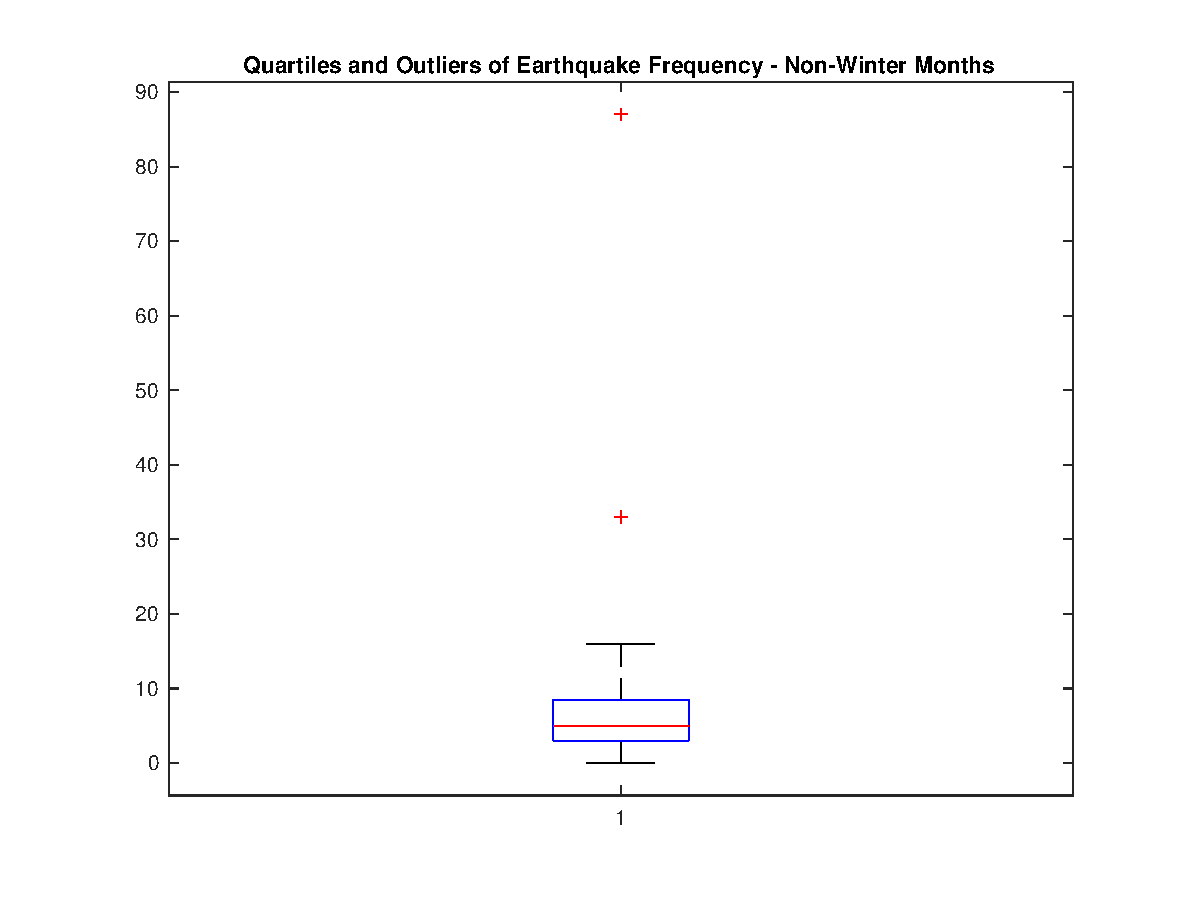
\includegraphics[scale=0.55]{boxplotfinal}
\caption{Box and whisker plot of thirty-day earthquake counts during non-winter months.\label{F:BoxAndWhiskerEarthquake}}
\end{figure}

\begin{figure}
\centering
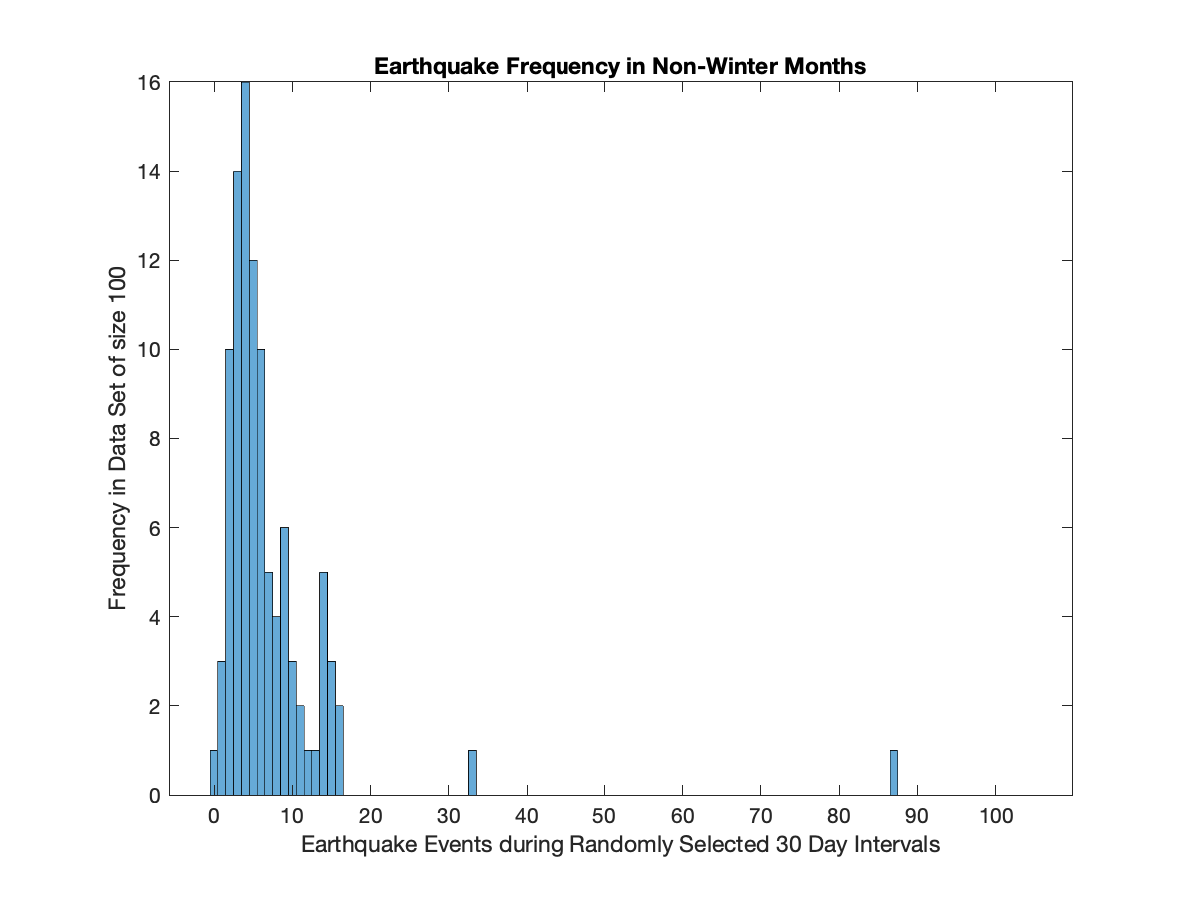
\includegraphics[scale=0.55]{histogramfinal}
\caption{Absolute frequencies of thirty-day earthquake counts during non-winter months.\label{F:absoluteFrequencies}}
\end{figure}

\section{A Model for Data Collection}
We built our control data set by randomly establishing 100 different 30 day intervals within the non winter months of the years 2000-2020 and counting the number of earthquakes recorded in the USGS data set that occurred during these intervals. Since we are measuring the frequency of an outcome (an earthquake) relative to a standardized interval, a reasonable course of action seems to be to model our control data with a Poisson framework. Our data can (in principle) take on any nonnegative integer value, so our sample space is the set $$\Omega=\{x: 0\le x\le \infty\},$$  where $x$ represents the number of earthquakes observed during a selected 30 day interval.  This sample space is countably infinite. We may organize the measurable events of our probability space into a $\sigma$-algebra $S$ by forming the power set, or set of all subsets, of the sample space.  There will be an uncountably infinite number of events in $S$. Finally, the Poisson framework uses the Poisson distribution to assign probabilities to the outcomes in $\Omega$:
\[
P(\lambda;x)=e^{-\lambda}\frac{\lambda^x}{x!}.
\]
Here, $\lambda$ represents the average number of earthquakes we \textsl{expect} to observe during a 30 day interval of non-winter months. This distribution predicts the probability of observing any value $x$ from our sample space. We may use it to compute the probability of any event $E$ in $S$ by summing the probabilities of each outcome in $E$:
\[
P(E)=\sum_{x\in E} P(\lambda;x).
\]
As such, the Poisson distribution generates the probability measure of the probability space that models our data collection approach. However, in order to make use of this distribution in this way, we will need to be able to measure or estimate the unknown parameter $\lambda$.
\section{Derivation of a Theoretical Distribution through Parameter Estimation}
As already stated, in order to model our data collection with the Poisson distribution, we will need to estimate the parameter $\lambda$. Recall $\lambda$ represents represents the average number of earthquakes we \textsl{expect} to observe during a 30 day interval of non-winter months. We estimated $\lambda$ by applying maximum likelihood estimation to $D_{control}$. This resulted in the value
\[
\lambda\simeq 7.14.
\]
Next, we turn to validating the Poisson model with this parameter value using both qualitative and quantitative techniques. If we plot the graph of expected frequencies predicted by this theoretical distribution on the same axes as the histogram of our control data (see figure \ref{F:graphicalAssessement}), we can see that agreement between the two appears to somewhat marginal. The observed freqeuencies found in the contrl data appear to be biased to the left of the expected frequencies. In addition, there appears to be both some high frequency outliers and a secondary peak of high frequency observations in the control data that do not appear in the expected frequencies. This might indicate poor agreement between the model and the control data.
\begin{figure}
\centering
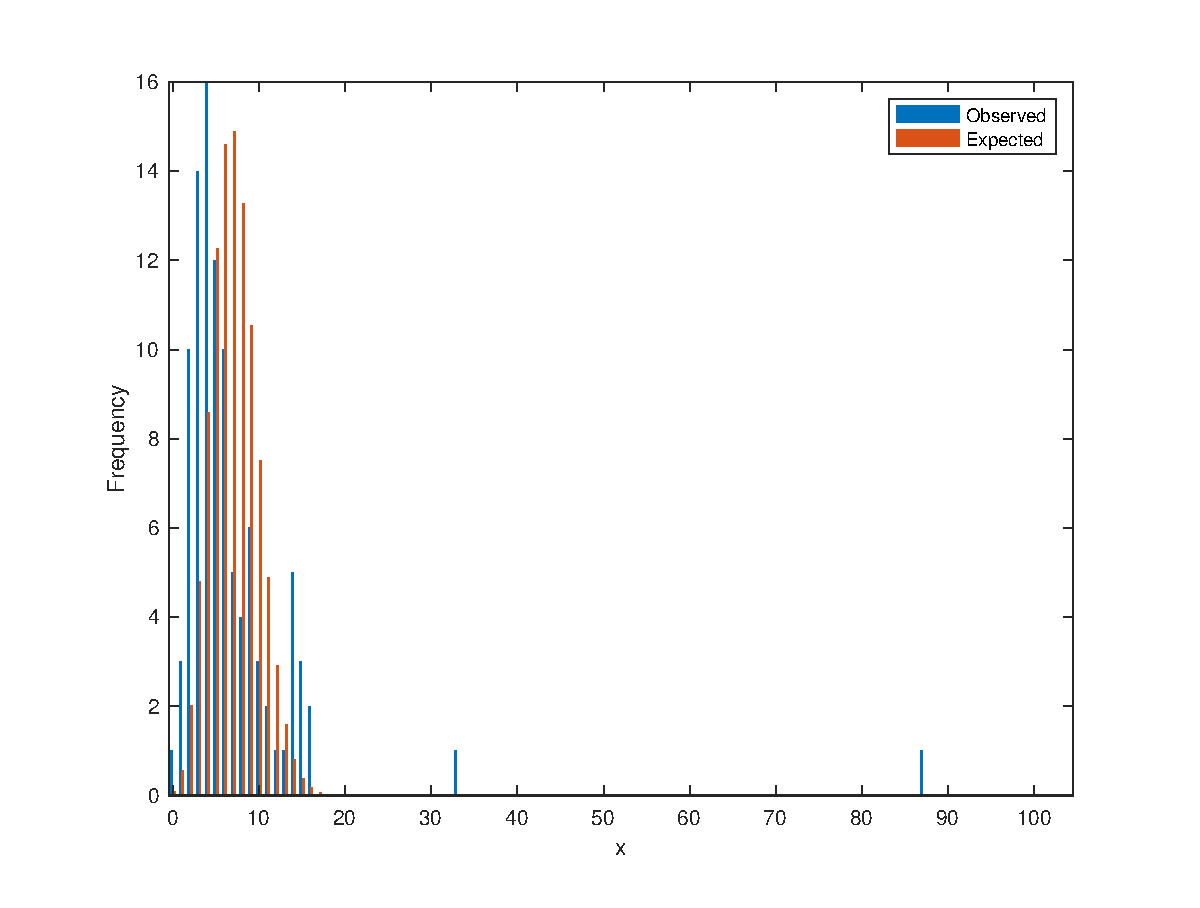
\includegraphics[scale=0.55]{histvalidationfinal}
\caption{
Comparison between empirical relative frequencies and theoretical, Poisson model.\label{F:graphicalAssessement}}
\end{figure}
We can also assess the fit of our model to the control data by computing the theoretical values of mean, variance, skewness, and kurtosis of our Poisson model and comparing them to the values we have already computed for our control data set. This comparison is summarized in Table \ref{Tbl:quantitativeAssessment}.
\begin{table}
\begin{tabular}{lrrrr}
\toprule
			&	{\bf Mean}	&	{\bf Variance}	&	{\bf Skewness}	&	{\bf Kurtosis}\\\midrule
{\sl Empirical}	&	7.14	&	86.5404	&	6.5533		&	54.9833\\ 
{\sl Theoretical}&	7.14	&	7.14		&	0.3742		&	3.1401\\
\bottomrule
\end{tabular}
 \caption{Quantitative comparison of the theoretical shape parameters of the Poisson model distribution to the empirical shape parameters of the control data set.\label{Tbl:quantitativeAssessment}}
\end{table}
Again, agreement between the empirical and theoretical shape parameter values is not great. In particular, it appears that the control data is much more variable than expected, it is more asymmetric (right-skewed, to be specific) than expected, and exhibits a much greater importance of outliers than expected.

Another fit assessment we can perform is to construct a quantile-quantile plot, or QQ plot, in which we plot the quantiles of each data point in $D_{control}$ against the theoretical quantiles of the Poisson distribution. When the distribution fits the data well, the QQ plot should show a linear relationship between the empirical and theoretical quantiles. Our QQ plot is displayed in figure \ref{F:qqplot}, and it is evident that such a linear relationship exists for the low-frequency part of the sample space, but breaks down in the higher frequency region. This is yet another indication that our model fits our data somewhat poorly.
\begin{figure}
\centering
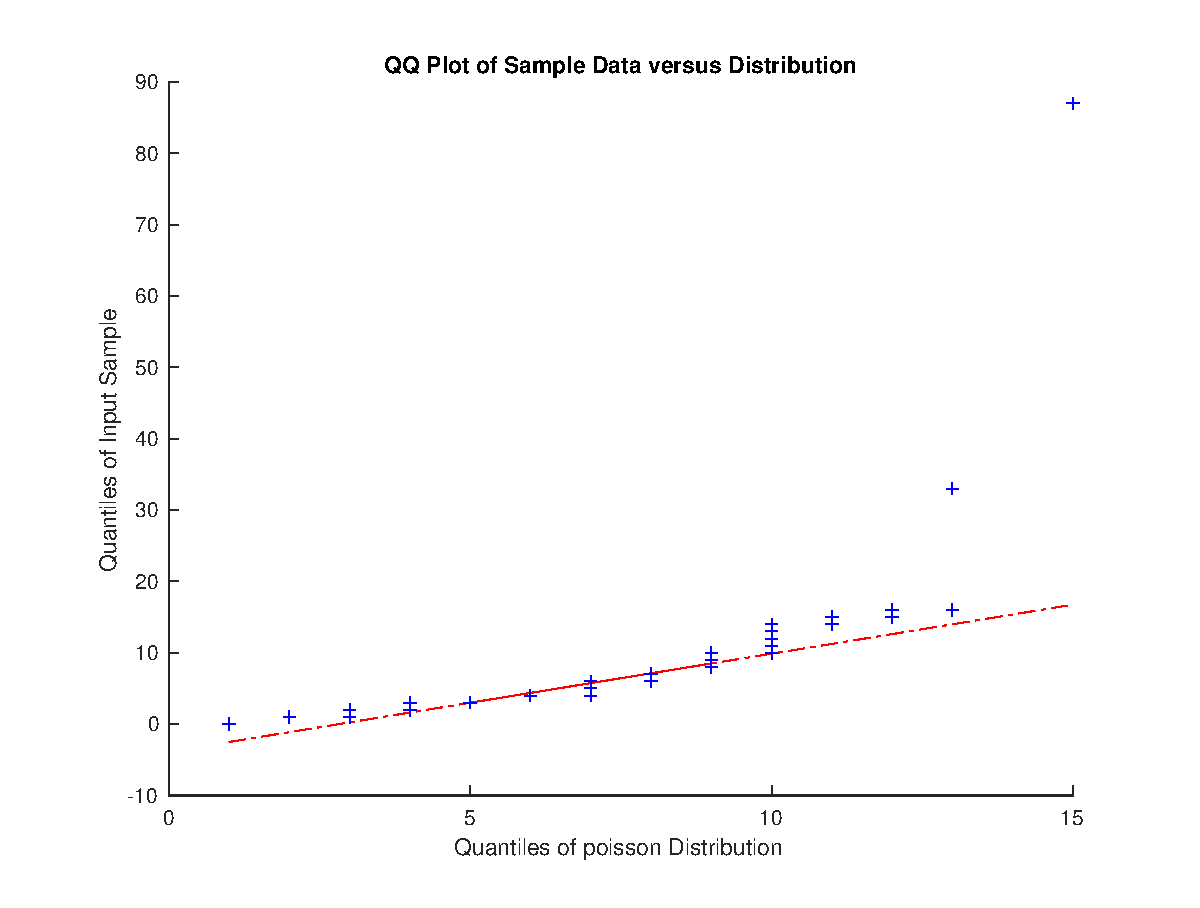
\includegraphics[scale=0.55]{qqplotfinal}
\caption{
Quantile-quantile plot expressing the relationship between the observed quantiles of each point in $D_{control}$ and the theoretical quantiles of the Poisson distribution.\label{F:qqplot}}
\end{figure}

Finally, we can be more quantitative still in comparing the data to the Poisson model by performing a goodness of fit test.  To do so, we pool the possible values from the sample space into bins that ensure there is an expected frequency ($E$) (predicted by the Poisson distribution) of at least 5 observations per bin.  Then, we compare these predictions to the actual frequencies observed ($O$) in these bins in our data set.  This information is summarized in the Table \ref{Tbl:chi2}.

\begin{table}
{\footnotesize
\begin{tabular}{lccccc}
\toprule
\multirow{2}{*}{Frequencies} & \multicolumn{3}{c}{Bins}\\	
	& $0\le x\le 4$ &	$4<x\le 8$ & 	$8<x\le \infty $ \\
	\midrule
Observed& 44& 31& 25\\
Expected & 16.0599& 55.0066& 28.9336\\
\bottomrule
\end{tabular}}
\caption{Expected and observed frequencies of earthquakes occurring during 30 day intervals within the non-winter months.\label{Tbl:chi2}}
\end{table}

From this data, we may compute the $\chi^2$ test statistic.
$$\chi^2=\sum\frac{(E(x)-O(x))^2}{E(x)}=59.6207$$
In order to compare this to an appropriate chi squared distribution, we need to determine the number of degrees of freedom for the comparison of our frequencies.  We have organized our frequencies into 3 bins.  However, in order to compute the expected frequencies, we used the Poisson distribution with an estimated value for $\lambda$.  We also are assigning three frequency counts out of a total of 100 observations to three bins. This means that there are $\nu$=3 bins-1 estimated parameter-1 dependency=1 degree of freedom. According to the $\chi^2$ distribution with $\nu=1$ degrees of freedom, the probability of observing a $\chi^2$ statistic at least as high as ours is
$$P(\chi^2\ge 59.6207;\nu=1)=1.1502\times 10^{-14}.$$
This value is small enough to reject the null hypothesis that states our model fits our control data well, so we conclude that the expected frequencies predicted by the Poisson distribution fit the data we've collected poorly.

All of our approaches to validating our Poisson model seem to agree that it falls short of describing our control data well. Specifically, it appears that there are some large outliers in the control data that cause it to be more right skewed and variable than expected. For this reason, we should be cautious about drawing any serious conclusions from any future hypothesis tests that rely heavily upon the notion that the Poisson distribution fits our control data well.
\section{Hypothesis Testing: Impacts of Seasonality upon Earthquake Frequency}
Our aim has been to determine if there is a relationship between seasonality and earthquake frequency. In particular, we hoped to determine if there is a significant difference in the frequency of earthquakes occurring during winter months compared to non-winter months. We had hoped to devise a Poisson model for earthquake frequency during non-winter months. This model would have described the expected behavior of our control population in hypothesis tests such as the Poisson test or the one sample t test. However, since it is clear from our validation that the Poisson model failed to adequately fit the control data, we will not rely upon those tests. Instead, we will rely only on test that look for differences between statistics of the control and experimental samples themselves, such as the two sample t test and a test for differences between two bootstrap samples.

The two sample t-test for determining if there is a significant difference between the means of the experimental and control data sets has at least three advantages for our application. First, this approach does not require us to assume any knowledge of the theoretical mean (or the corresponding theoretical distribution) of the population the control data set was sampled from. Second, the two sample t-test is a little more conservative than the one sample test, so if are able to establish significance with it, then we are doing so in a rather grounded way. Finally, the two sample gives us the option of relaxing any assumptions about the equality between the variances of the  experimental and control populations. We don't have any \textsl{a priori} knowledge of whether those variances are similar, but we can check by applying the F test to our control and experimental sample. This results in a p value of $p_F=1.2065 \times 10^{-14}$ for evaluating the null hypothesis:
\begin{description}
\item[$H_{0,F}$] There is no significant difference between the variance of the experimental data set and the variance of the control data set.
\end{description}.
Since $p_F$ is well below a threshold of 5\%, we may reject $H_{0,F}$ and proceed with the two sample t-test for determining if there is a difference between means of two samples of unequal variance. The null hypothesis for the two sample t-test is
\begin{description}
\item[$H_{0,T}$ (null hypothesis)] There is no significant difference between the means of the experimental and control data sets.
\end{description}
When we applied the two sample t-test to our control and experimental samples, we achieved a p-value of $p_T=0.5323$, so we have insufficient evidence for rejecting $H_{0,T}$ -- we have no reason to believe that there is a meaningful difference in the average frequency of earthquakes in winter months compared to the average frequency during non winter months. This test also returned a 95\% confidence interval for the location of the difference between the true means of the experimental and control populations: $-2.6613\le \bar{x_E}-\bar{x_C} \le -1.3813$.
The true difference between the means is $\bar{x_E}-\bar{x_C}=-0.64$. This falls well within the confidence interval, which is another indicator that there isn't much difference between the means.

An alternate approach for investigating differences between the experimental and control means is to construct bootstrap samples from our experimental and control data and test for differences between \textsl{their} means by computing the achieved significance level (ASL). This will serve in place of a p-value, but it also provides us with a synthetic way of establishing confidence intervals for both our experimental and control means that will give us some indication of range of possible results for our experiment if we were to have replicated it multiple times. We constructed 2000 bootstrap samples each from our control and experimental data sets by repeatedly sampling 100 values from them \textsl{with replacement}. We tracked the mean and standard deviation of these samples so that we could compute a t statistic for each pair of bootstrap samples. We found the ASL by computing the percentage of these t statistics that were larger than the true t statistic computed from our original experimental and control data sets. This resulted in a value of $ASL=0.7795$. This is well enough above 5\% that it does not cause us to suspect there is a difference between our experimental and control means. Moreover, we can estimate a pair of 95\% confidence intervals for predicting the location of the means of the populations our experimental and control data were sampled from by computing the 97.5\% and 2.5\% quantiles of the two bootstrap samples. We've displayed these confidence intervals, together with the means of the experimental and control data sets on top of the histograms of the experimental and control bootstrap samples in figure \ref{F:bootstrap}.
\begin{figure}[H]
\centering
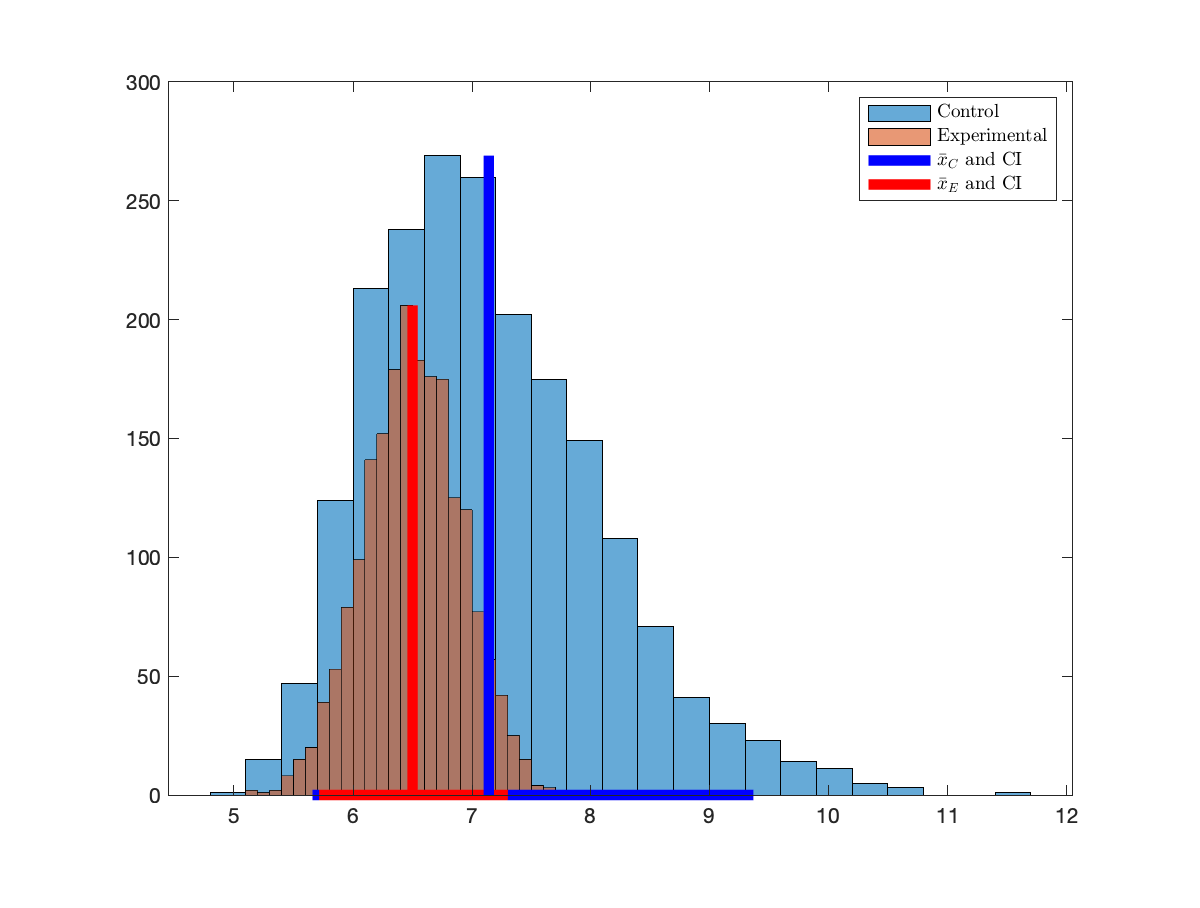
\includegraphics[scale=0.55]{bootstrapTwoSample}
\caption{
Histograms of experimental and control bootstrap samples are displayed with the means of the experimental and control samples as well as the approximate 95\% confidence intervals for the location of the means of the populations that the experimental and control data were sampled from. The means of the experimental and control samples fall within the intersection of the two confidence intervals.\label{F:bootstrap}}
\end{figure}
The fact that the means of the experimental and control samples fall within the intersection of the two confidence intervals indicates that it is likely that replication of this experiment would reproduce our non-significant result with great consistency.
\section{Conclusion}
In this initial study, we were interested in determining whether we could find evidence consistent with the hypothesis that there is a difference in earthquake frequency during winter months compared to non-winter months. We have collected 
100 separate 30-day counts of earthquakes during non-winter months (our control data set) and 100 separate 30-day counts of earthquakes during winter months. All counts were obtained from reports of earthquakes of magnitude 4.0 or greater in the conterminous US during the years of 2000-2020. We attempted to fit a Poisson model to the control data, but all of our validation techniques indicated that this model did not fit the data well. For this reason, we restricted our methods of hypothesis testing to a two-sample t test and a achieved significance level(ASL) analysis of 2000 bootstrap samples of means collected from the control data set (and 2000 more collected from the experimental data). Neither of these techniques indicated that there is a significant difference between winter and non-winter thirty-day earthquake counts, and the bootstrap analysis suggested that this result would appear consistently were we to replicate our experiment.
\end{document}
